%!TEX TS-program = xelatex
%!TEX encoding = UTF-8 Unicode
%!TEX options=--shell-escape 

\documentclass[dsingle]{memo}

% \nobibliography*

%!TEX root = dissertation.tex

\newcommand{\figref}[3][Figure~]{#1\hyperref[#2]{\ref*{#2}\textsc{#3}}}
\newcommand{\subcap}[1]{\textcolor{graylink}{\textbf{(#1)}}}
\newcommand{\captiontitle}[1]{\textit{\textbf{#1}}}

\newcommand{\separator}{%
\begin{center}
  $\ast$~$\ast$~$\ast$
\end{center}
}

\newcommand{\juliacode}[1]{
  \inputminted[
    mathescape=true,
    fontsize=\small,
    frame=lines,
    framesep=2mm,
  ]{julia}{#1}
}
\newcommand{\tmax}{N}

\newcommand{\A}{\mathcal{A}}
\newcommand{\C}{\mathcal{C}}
\newcommand{\B}{\mathcal{B}}
\newcommand{\D}{\mathcal{D}}
\renewcommand{\O}{\mathcal{O}}
\renewcommand{\S}{\mathcal{S}}
\newcommand{\R}{\mathbb{R}}
\newcommand{\Z}{\mathbb{Z}}
\newcommand{\W}{\mathcal{W}}
\newcommand{\M}{\mathcal{M}}


% \newcommand{\expect}[2][]{\mathbb{E}_{#1} \left[ #2 \right]}
\newcommand{\Normal}{\mathrm{Normal}}
\newcommand{\Uniform}{\mathrm{Uniform}}
\renewcommand{\vec}[1]{\mathbf{#1}}
\newcommand{\meta}{_{\text{meta}}}
\newcommand{\greedy}{_{\text{greedy}}}
\newcommand{\object}{_{\text{object}}}
\newcommand{\act}{_{\text{act}}}
\newcommand{\cost}{\text{cost}}
\newcommand{\utility}{\text{utility}}
% \newcommand{\considered}{_{\text{con}}}
\newcommand{\considered}{_c}
\newcommand{\other}{_{\text{other}}}

\newcommand{\w}{\vec{w}}

\DeclareMathOperator*{\argmax}{argmax}
\DeclareMathOperator*{\argmin}{argmin}
\DeclareMathOperator*{\E}{E}
\DeclareMathOperator*{\Var}{Var}

% \newcommand{\argmax}[1]{\underset{#1}{\operatorname{argmax}}\;}


\newcommand{\fix}{\marginpar{FIX}}
\newcommand{\new}{\marginpar{NEW}}
\newcommand{\red}[1]{\textcolor{red}{#1}}
\newcommand{\todo}[1]{\textcolor{red}{TODO: #1}}
\newcommand{\tocite}{\textcolor{red}{[citation]}}

\newcommand{\expect}[2]{\E \left[ #1 \ \middle\vert\ #2 \right]}
\newcommand{\expectunder}[2]{\E_{#2} \left[ #1 \right]}

\newcommand{\curly}[1]{\left\{ #1 \right\}}


% ATTENTION
\newcommand{\given}{\bigm\vert}
\newcommand{\last}{f}
\newcommand{\std}{\operatorname{std}}
\newcommand{\mean}{\operatorname{mean}}
\newcommand{\cdf}{\operatorname{cdf}}

\newcommand{\nop}{\texttt{NOOP}}
\newcommand{\samplecost}{\gamma_\text{sample}}
\newcommand{\switchcost}{\gamma_\text{switch}}
\newcommand{\pswitch}{p_\text{switch}}
\newcommand{\pstop}{p_\text{stop}}
\newcommand{\sampletime}{t_\text{sample}}

\newcommand{\VOC}{\text{VOC}}
\newcommand{\VOI}{\text{VOI}}
\newcommand{\VOImy}{\VOI_\text{myopic}}
\newcommand{\VPIitem}{\VOI_\text{item}}
\newcommand{\VPI}{\VOI_\text{full}}
\newcommand{\VOCapprox}{\widehat{\text{VOC}}(b, c; \vec{w})}
\newcommand{\VOChat}{\widehat{\text{VOC}}}
\newcommand{\like}{\mathcal{L}(D \mid \theta)}

% PLANNING


\newcommand{\norm}[1]{\left\lVert#1\right\rVert}

\renewcommand{\P}{\mathcal{P}}

\newcommand{\rmeta}{r\meta}
\newcommand{\tmeta}{T\meta}
\newcommand{\term}{\bot}
\newcommand{\pselect}{p_{\mathrm{select}}(s, a)}
\newcommand{\myopic}{^{\mathrm{myopic}}}
\newcommand{\bmps}{^{\mathrm{bmps}}}

\renewcommand{\stop}{_{\mathrm{stop}}}
\newcommand{\select}{_{\mathrm{select}}}
\newcommand{\depth}{_{\mathrm{depth}}}
\newcommand{\frontier}{\mathrm{frontier}}
\newcommand{\bias}{\psi_\mathrm{forward}}
\newcommand{\prune}{_{\mathrm{prune}}}
\newcommand{\dnll}{\Delta_{\mathrm{LL}}}

\newcommand{\best}{_{\mathrm{best}}}
\newcommand{\nxt}{_{\mathrm{next}}}
\newcommand{\satisfice}{_{\mathrm{satisfice}}}


% \newcommand{\heur}{^{H}}
% \newcommand{\opt}{^{O}}
% \newcommand{\greedy}{^{G}}

\newcommand{\phiopt}{\phi^{\mathrm{opt}}}
\newcommand{\phimg}{\phi^{\mathrm{MG}}}
\newcommand{\phiclass}{\phi^{\mathrm{heur}}}
\newcommand{\phirand}{\phi^{\mathrm{rand}}}
\newcommand{\expp}[1]{\exp\left\{#1\right\}}






\title{Pr\'ecis of \emph{Cognition as a sequential decision problem}}
\author{Frederick Callaway}
\date{}

\begin{document}

\setstretch{\dnormalspacing}

\maketitle

\begin{quote}
\emph{We must be prepared to accept the possibility that what we call
``the environment'' may lie, in part, within the skin of the biological
organism.} ---Herb Simon \citeyearpar{simon1955behavioral}
\end{quote}

How can we build theoretically satisfying and practically useful models of the human mind? Historically, there have been two broad approaches. The \emph{rational} approach, exemplified by \citet{anderson1990adaptive}, focuses on characterizing the problems people have to solve and the optimal solutions to those problems. Under the assumption that the mind is well adapted to its environment, these optimal solutions then serve as models of cognition. Rational models are satisfying because they tell us \emph{why} the mind works the way it does, and they are useful because they allow us to make generalizable predictions about how people will behave in new environments (i.e., rationally). However, by construction, such models don't explain \emph{how} the mind achieves the rational ideal, and a growing list of systematic cognitive biases \citep{kahneman2011thinking} draws their predictive utility into question.

In contrast, the \emph{mechanistic} approach focuses on identifying the cognitive processes underlying behavior, often with an emphasis on explaining the behavioral idiosyncrasies that rational models gloss over. This approach can potentially tell us how the mind actually works, and it can produce extremely accurate models. However, lacking the optimality constraint, there is an enormous space of possible mechanistic models, and they often have many free parameters that are tuned for specific experimental setups. We are thus left wondering why this specific model fit the data best, and whether it would continue to make good predictions in a slightly different context.

Although the rational and mechanistic approaches have traditionally been viewed as conflicting, the past decade has seen a resurgence of an old idea \citep{simon1955behavioral}: rationality can be seen as a property of cognitive mechanisms themselves. Specifically, a cognitive mechanism is rational if it makes optimal use of limited cognitive resources. Going under various names---cognitively bounded rational analysis \citep{howes2009rational}, computational rationality \citep{lewis2014computational,gershman2015computational}, and resource-rational analysis \citep{griffiths2015rational,lieder2020resourcerational} to name a few---this view suggests that we should not expect people to be rational in the traditional sense of taking actions that maximize expected utility \citep{vonneumann1944theory}. Instead, we should expect people to select actions using mental strategies that strike a good tradeoff between the utility of the chosen action and the cognitive cost of making the decision.

But what defines a ``good'' tradeoff between action utility and cognitive cost? And how can we identify mental strategies that achieve such a tradeoff? In my dissertation, I suggest answers to these questions based on a key insight: \emph{a rational mental strategy is one that optimally solves the sequential decision problem posed by one's internal computational environment}. Under this view, cognition is a problem of stringing together a series of basic cognitive operations, or ``computations'', in the service of choosing what to do in the world. An optimal cognitive process strings those basic operations together in such a way that maximizes the difference between the utility of the ultimate behavior and the total cost of all the cognitive operations that support the behavior.

The dissertation consists of six chapters. In the first chapter, I introduce the idea that cognition is a sequential decision problem, and provide theoretical context motivating my formalization of this idea. In the second chapter, I give a complete specification of that formalization using the framework of \emph{metalevel Markov decision processes}. In the next three chapters, I illustrate how my colleagues and I have applied the framework to understand how people think about the present (attention), the past (memory), and the future (planning). In each case, we use process-tracing data to reveal in which ways people's cognitive processes are consistent with and different from optimal cognitive processes. Taken together, the results suggest that people's mental strategies are well-adapted to the limitations posed by their cognitive architectures, often in ways that could not be revealed without considering the sequential nature of cognition. In the final chapter, I identify ways in which the framework could be further developed.


\section{Chapters 1 and 2: Metalevel Markov decision processes}\label{formal-framework-metalevel-mdps}


\begin{figure}[tbp]
  \centering
  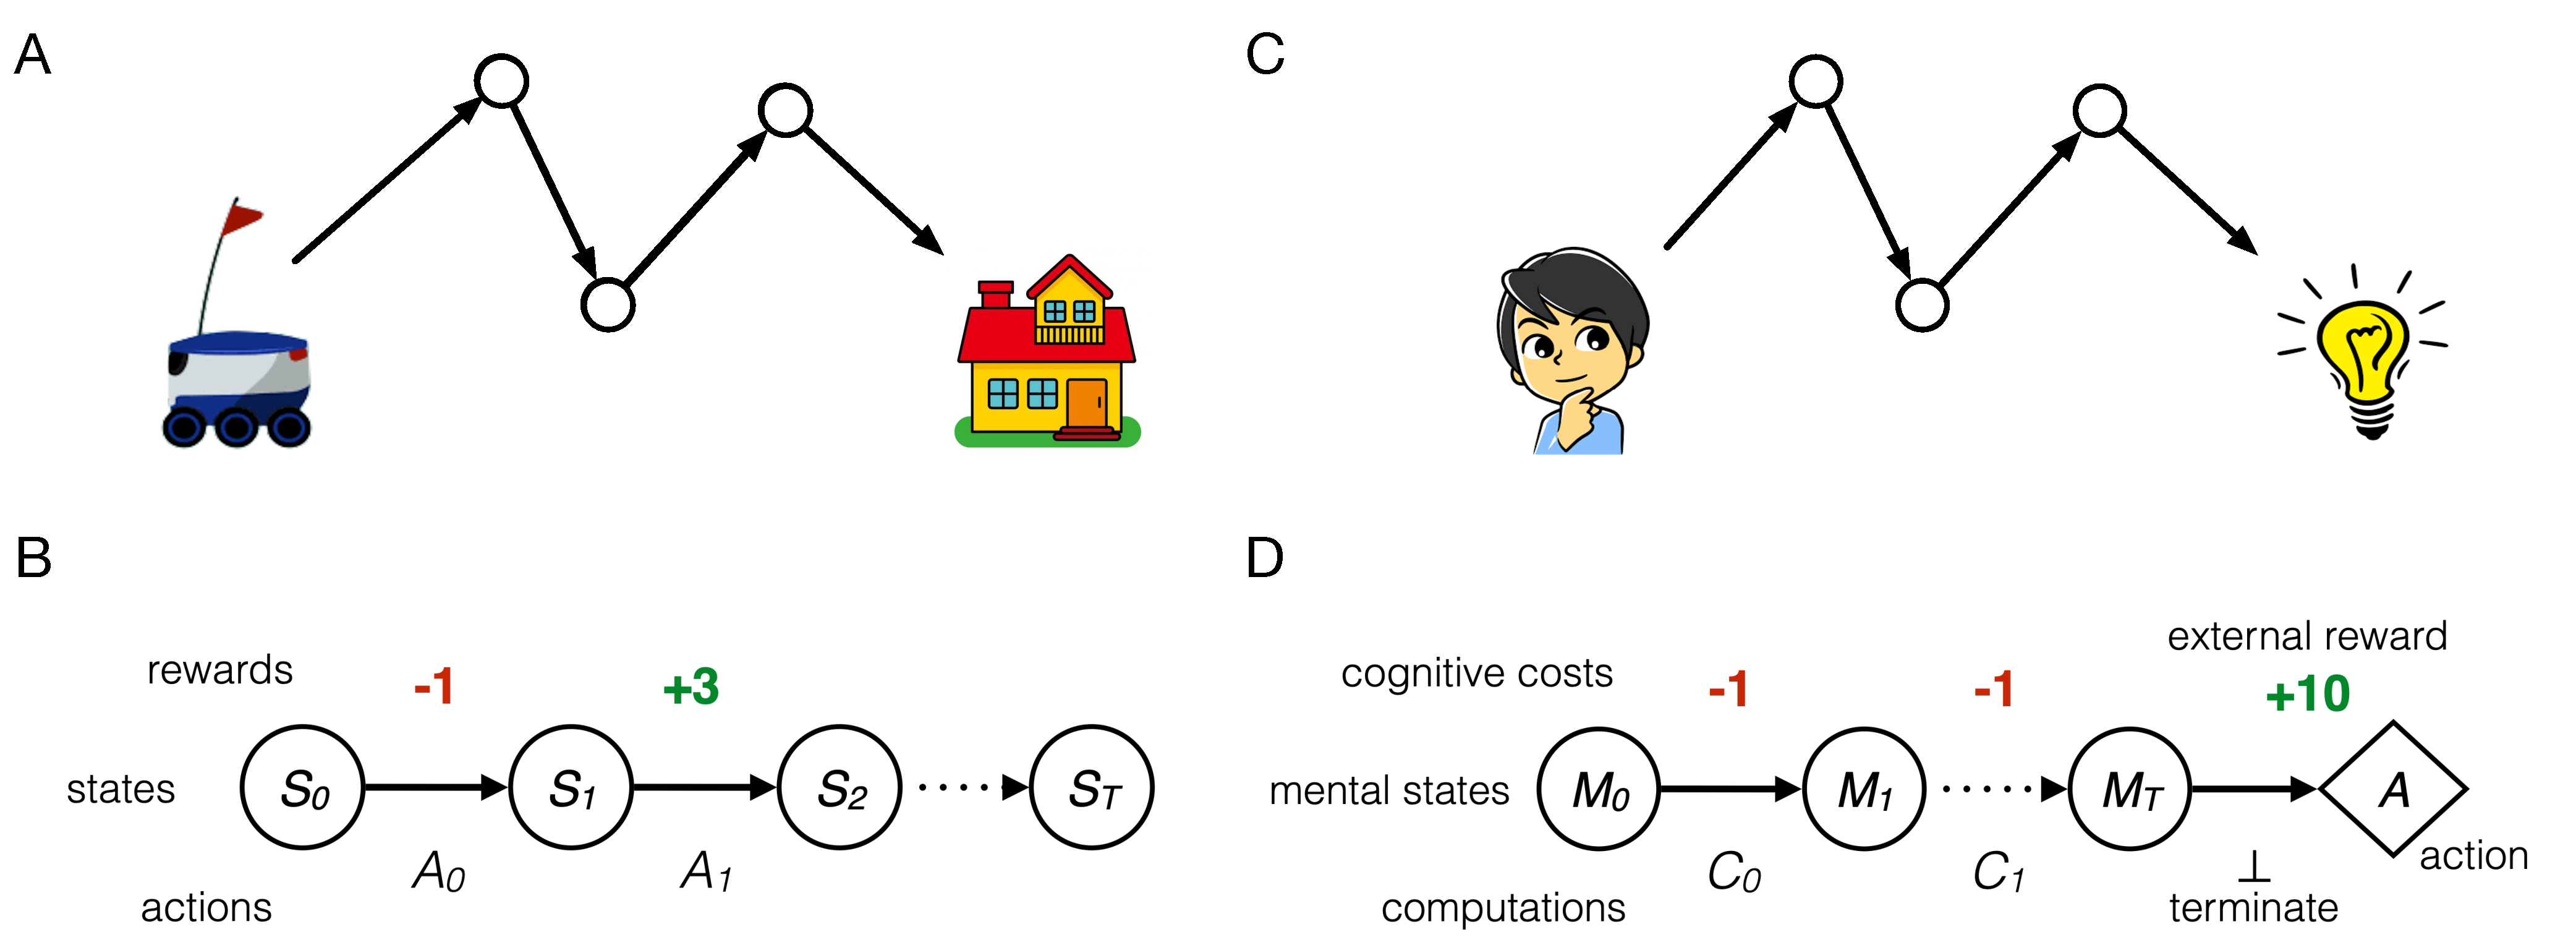
\includegraphics[width=\textwidth]{diagrams/precis/intro.pdf}
  \caption{Sequential decision problems posed by external and internal environments.}
  \label{fig:sequential-intuition}
\end{figure}

What does it mean to say that cognition is a sequential decision problem? One way to understand this claim is as an analogy between the type of problems posed by our external, physical environments and the type of problems posed by our internal, mental environments. To make things concrete, consider the problem facing a delivery robot, illustrated in \figref{fig:sequential-intuition}{a}. Completing the delivery will require visiting a sequence of locations before arriving at the final destination. And at each location, the robot will need to decide where to go next. Thus, the robot faces a sequential decision problem. \figref{fig:sequential-intuition}{b} illustrates how this type of problem is often modeled in artificial intelligence research: a \emph{Markov decision process}, or MDP. At each time step, an agent (here, the robot) takes an \emph{action} (e.g., driving forward). This action causes the environment to enter a new \emph{state} (e.g., one where the robot is in a new location). Additionally, the agent receives a \emph{reward}, a number that captures how good or bad the immediate consequences of the action are. For example, the delivery robot might receive a large positive reward for reaching the destination and a small negative reward every time it moves (capturing the desire to conserve battery life). The robot's goal is to maximize the total reward received.
% After receiving the reward and new state, the agent selects another action and the cycle continues.

\figref{fig:sequential-intuition}{c} illustrates a seemingly very different type of situation: a person trying to come up with a solution to a difficult problem. However, as the diagram suggests, the two cases actually share the same basic structure. Both involve an extended interaction between an agent and an environment; but whereas the robot is interacting with an \emph{external} environment, the thinker is interacting with an \emph{internal} environment: their own mind. Just as the robot makes several moves, and visits several locations before reaching the destination, the thinker has several thoughts, and enters several mental states before discovering the solution. Indeed, as illustrated in \figref{fig:sequential-intuition}{d}, this problem can be modeled in precisely the same way as the delivery problem. However, now the actions correspond to \emph{computations} and the states correspond to \emph{mental states}. Thinking changes one's mental state just as moving changes one's physical state; and it also incurs a cost---at the very least, thinking takes time. Because this MDP describes the metacognitive problem of how to interact with one's own mind, it is called a \emph{metalevel} MDP \citep{hay2016principles}.

The power of identifying this parallel between external and internal environments is that it allows us to leverage existing knowledge about solving MDPs (a substantial chunk of AI research) to build rational mechanistic models of cognition. By modeling the internal environment associated with some cognitive system as a metalevel MDP, we can identify the optimal cognitive process as the optimal policy for that MDP. In the next three chapters, I show how this provides insights about three domains of cognition.


\section{Chapter 3: Attention}

\begin{figure}[t!]
  \centering
  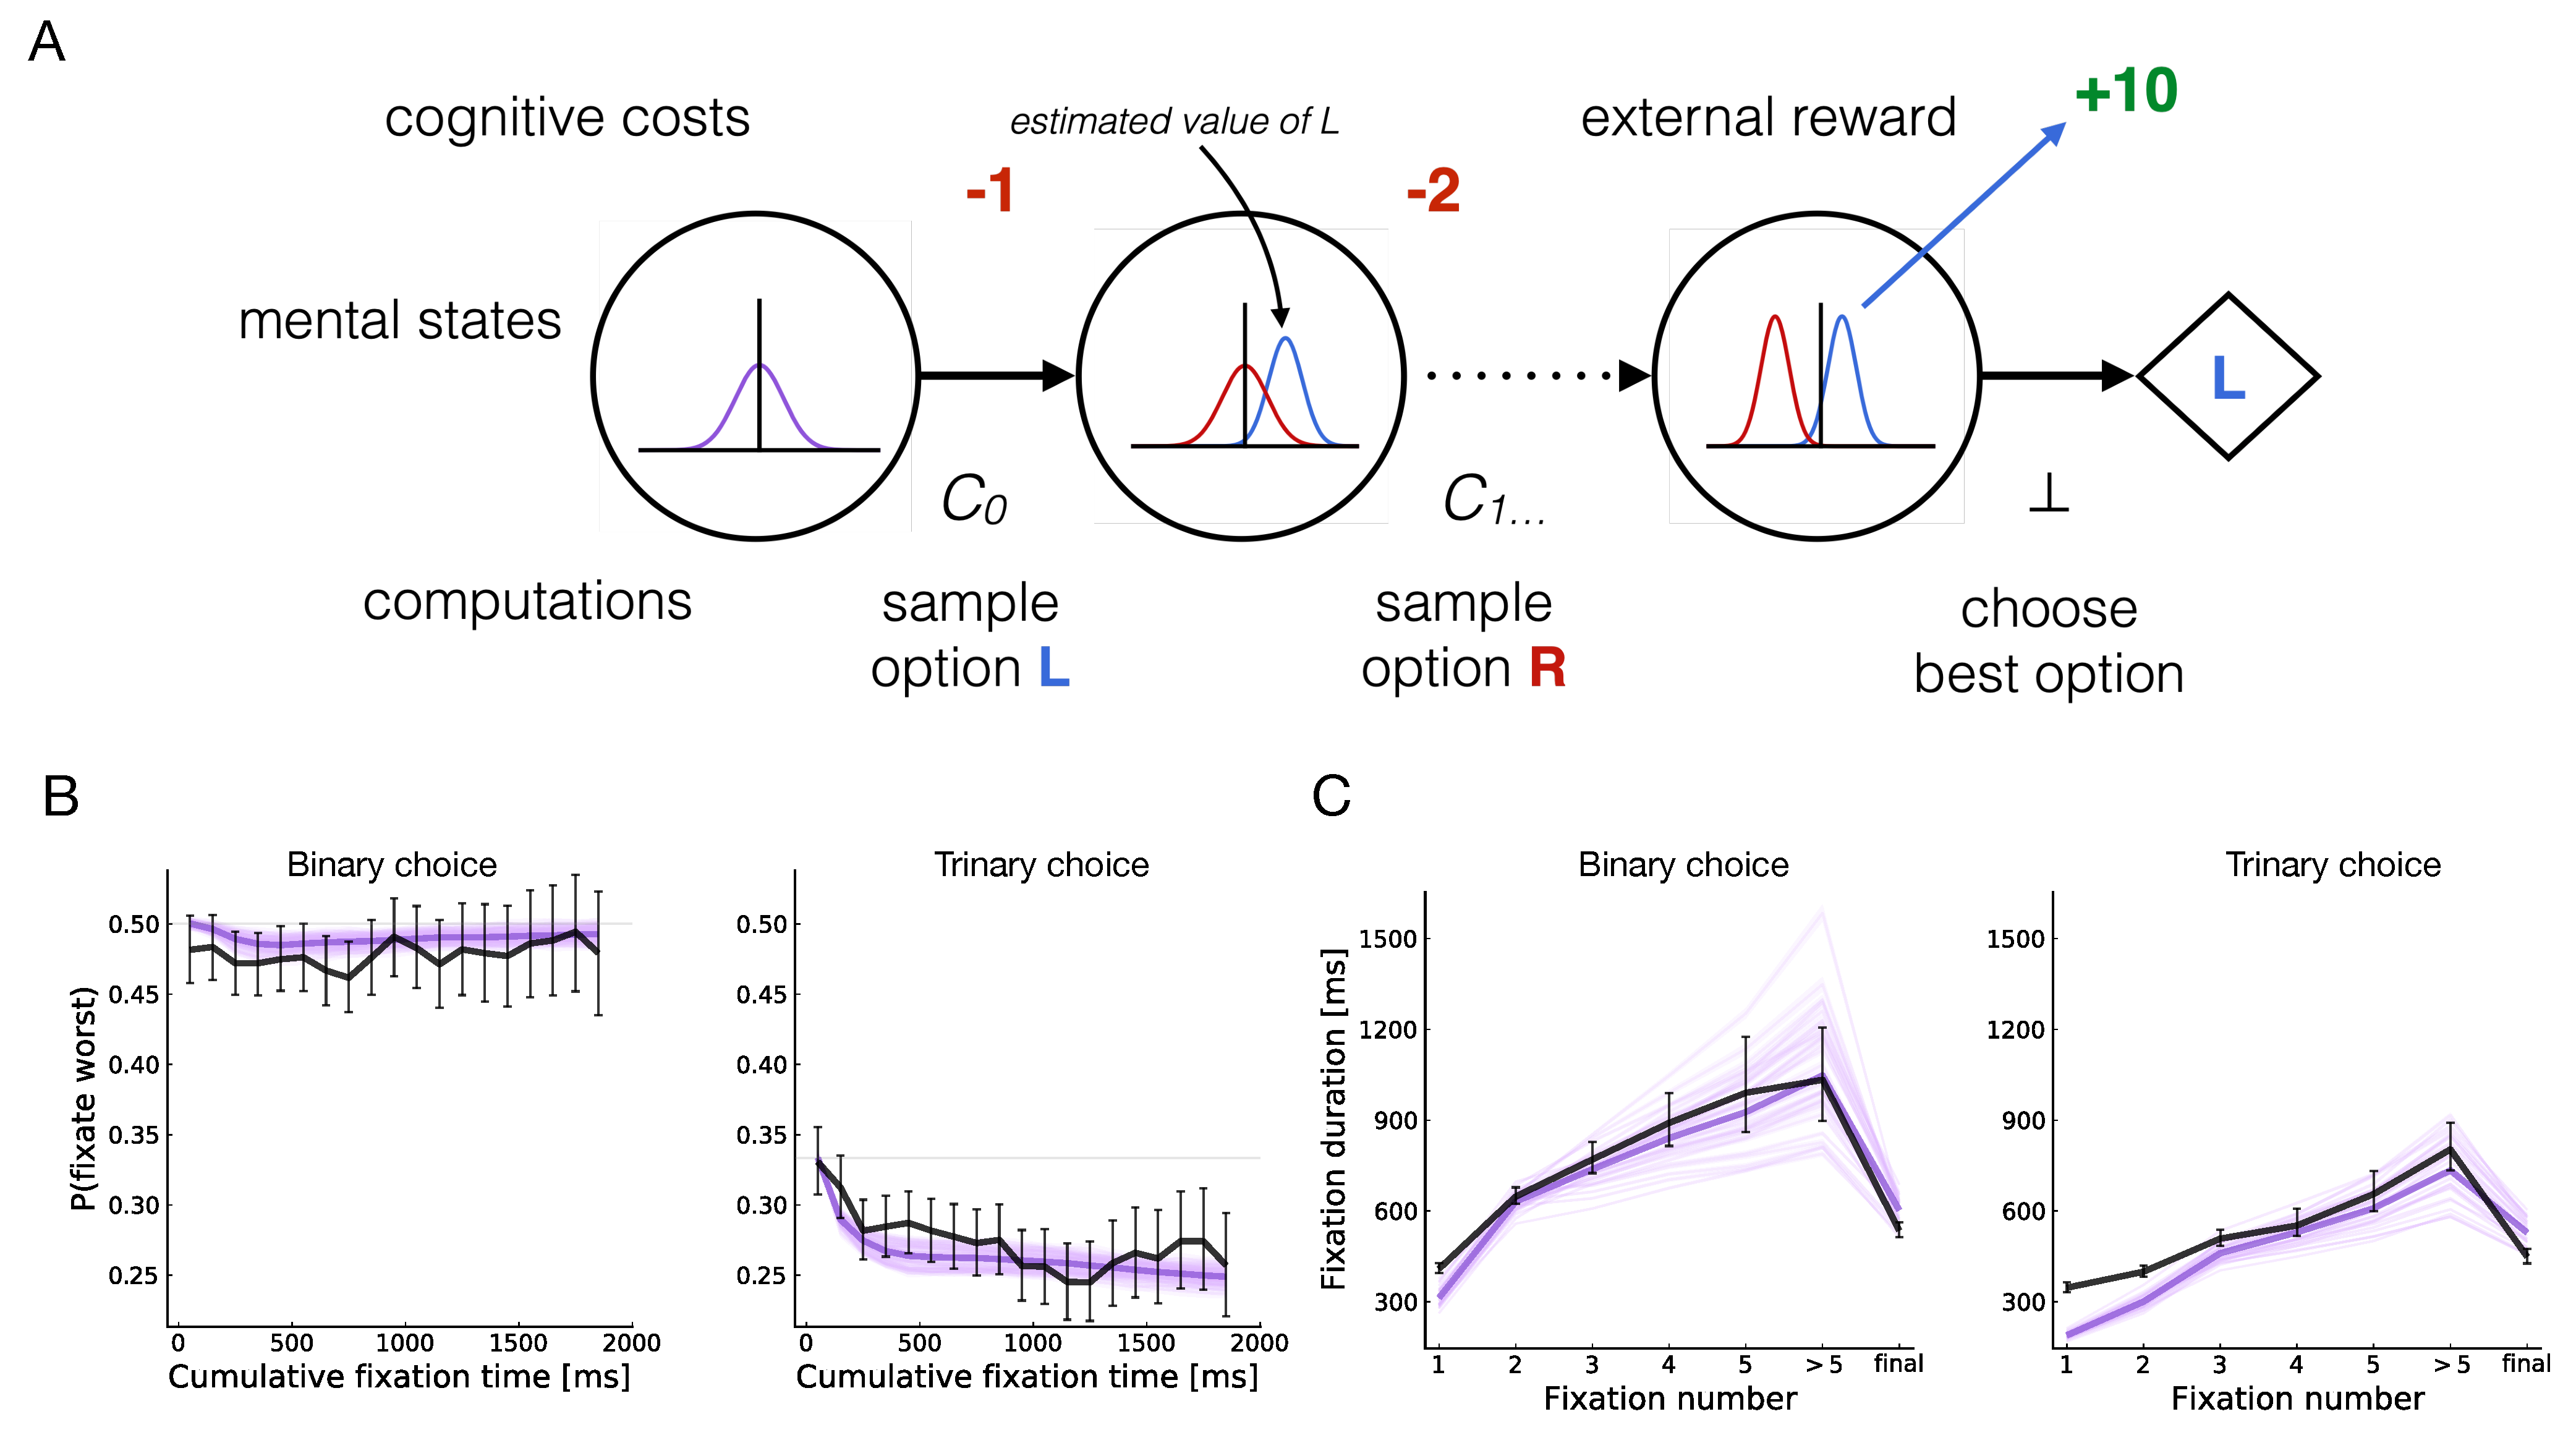
\includegraphics[width=\textwidth]{diagrams/precis/attention.pdf}
  \caption{\captiontitle{Attention}
    \subcap{A} Meta-level MDP. The mental state encodes a distribution over the value of each option in the choice set. A computation corresponds to sampling the value of an option and updating its estimated value by Bayesian inference.
    \subcap{B} Both people (black) and the model (purple) are equally likely to attend to the better or worse option in binary choice (left). In trinary choice however (right), they are less likely to attend to the worst option in the set as the decision progresses.
    \subcap{C} Both people and the model show increasing fixation durations over the course of a decision.
  }
  \label{fig:attention}
\end{figure}


Consider the problems faced by a diner at a buffet or a shopper at a supermarket shelf. They are presented with a number of options and must evaluate them until they identify the most desirable one. Previous work suggests that these decisions are made by integrating noisy evidence about the value of each alternative, which is sampled over time \citep{ratcliff2008diffusion,milosavljevic2010drift,usher2001time}. Moreover, this process is guided by visual attention, such that the evidence is strongest for the item currently being looked at; as a result, what we look at has consequences for what we choose \citep{shimojo2003gaze,armel2008biasing,krajbich2010visual}. This raise an important question: \textbf{How do we decide what to pay attention to when making decisions?}

This problem is naturally cast as a metalevel MDP (\figref{fig:attention}{a}). The mental states correspond to the agent's current estimates of (and uncertainty about) the value of each item. The computations correspond to attending to a given option, drawing a noisy sample of its value, and integrating that information into the corresponding value estimate by Bayesian inference. This sampling and updating process is encoded by the transition function. Finally, the reward function imposes a fixed cost for each sample, an additional switching cost for saccades, and a reward equal to the true value of the chosen option.

Solving the metalevel MDP yields an optimal policy for allocating attention when making decisions. We compare this policy with human attention allocation using two datasets in which participants chose between junk food snacks (either two or three per trial) while their gaze was recorded with an eye tracker \citep{krajbich2010visual,krajbich2011multialternative}. We can simulate this kind of data from the model by assuming that the attended item is fixated (100ms for each sample drawn). In the dissertation, I conduct a thorough comparison of optimal and human attention allocation in simple choice. Here, I highlight two of the most striking findings.

% As illustrated in \figref{fig:attention}{b}, the optimal policy is highly sensitive to two key features of the mental state: 1) uncertainty about the true values and (2) differences in the value estimates. In both binary and trinary choice, the policy prefers to sample from items with high uncertainty and whose estimated value is similar to the other items in the choice set. In the case of trinary---but not binary---choice, we additionally see a stark asymmetry in the effect of relative estimated value. While the policy is likely to sample from an item whose value is substantially higher than the competitors, it is unlikely to sample from an item with value well below. In particular, the policy has a strong preference to sample from the items with best or second-best value estimates. Intuitively, this is because sampling those items is most likely to change the choice one makes, by switching the order of the top two contenders.


\figref{fig:attention}{b} shows the probability of fixating on the worst option in the choice set over the course of a decision. When choosing between two items (left), both people (black) and the model (purple) are just about equally likely to fixate on the better and worse item throughout the decision. When choosing between three items, however, they are both decreasingly likely to look at the worst option as time goes on. Why do we see this pattern? Intuitively, when considering more than two options, one should focus on the top two contenders, as refining the value estimate for these options is most likely to change one's mind about which option is best---indeed, this is exactly what the optimal policy does. When there are only two options, they are by definition both in the top two, and thus there is no asymmetry. Furthermore, this effect emerges over time because attention must be allocated based on one's \emph{estimates} of value, which only become related to the items' true value after some information has already been sampled. 

% In the dissertation, I show that find similar patterns in the overall proportion of fixation and the duration of the first fixation. And in the trinary case, we also see an effect of value on the probability of refixating items, further confirming value-directed attention in this case.

To highlight a less intuitive prediction, \figref{fig:attention}{c} shows the duration of fixations over the course of a decision. Although the model tends to underpredict the duration of the first two fixations in the three-item case, it captures well three key patterns: (a) the final fixation is shorter, (b) later (but non-final) fixations are longer and (c) fixations are substantially longer in the two-item case. The first occurs because final fixations are cut off when a choice is made, as in previous evidence accumulation models \citep{krajbich2010visual}. The latter two patterns are unique predictions of the optimal model. They arise because more evidence is needed to alter beliefs when their precision is already high; this occurs late in the trial, especially in the two-item case where samples are split between fewer items.

Critically, these qualitative differences in the model predictions in binary and trinary choice are not the result of model fitting. The same set of parameters are used to generate predictions in each case, and the key qualitative differences are highly robust to the values of those parameters. This illustrates the power of rational models to generalize.

This work was published in \emph{PLoS Computational Biology} \citep{callaway2021fixation}.

\section{Chapter 4: Memory}

\begin{figure}[ph]
  \centering
  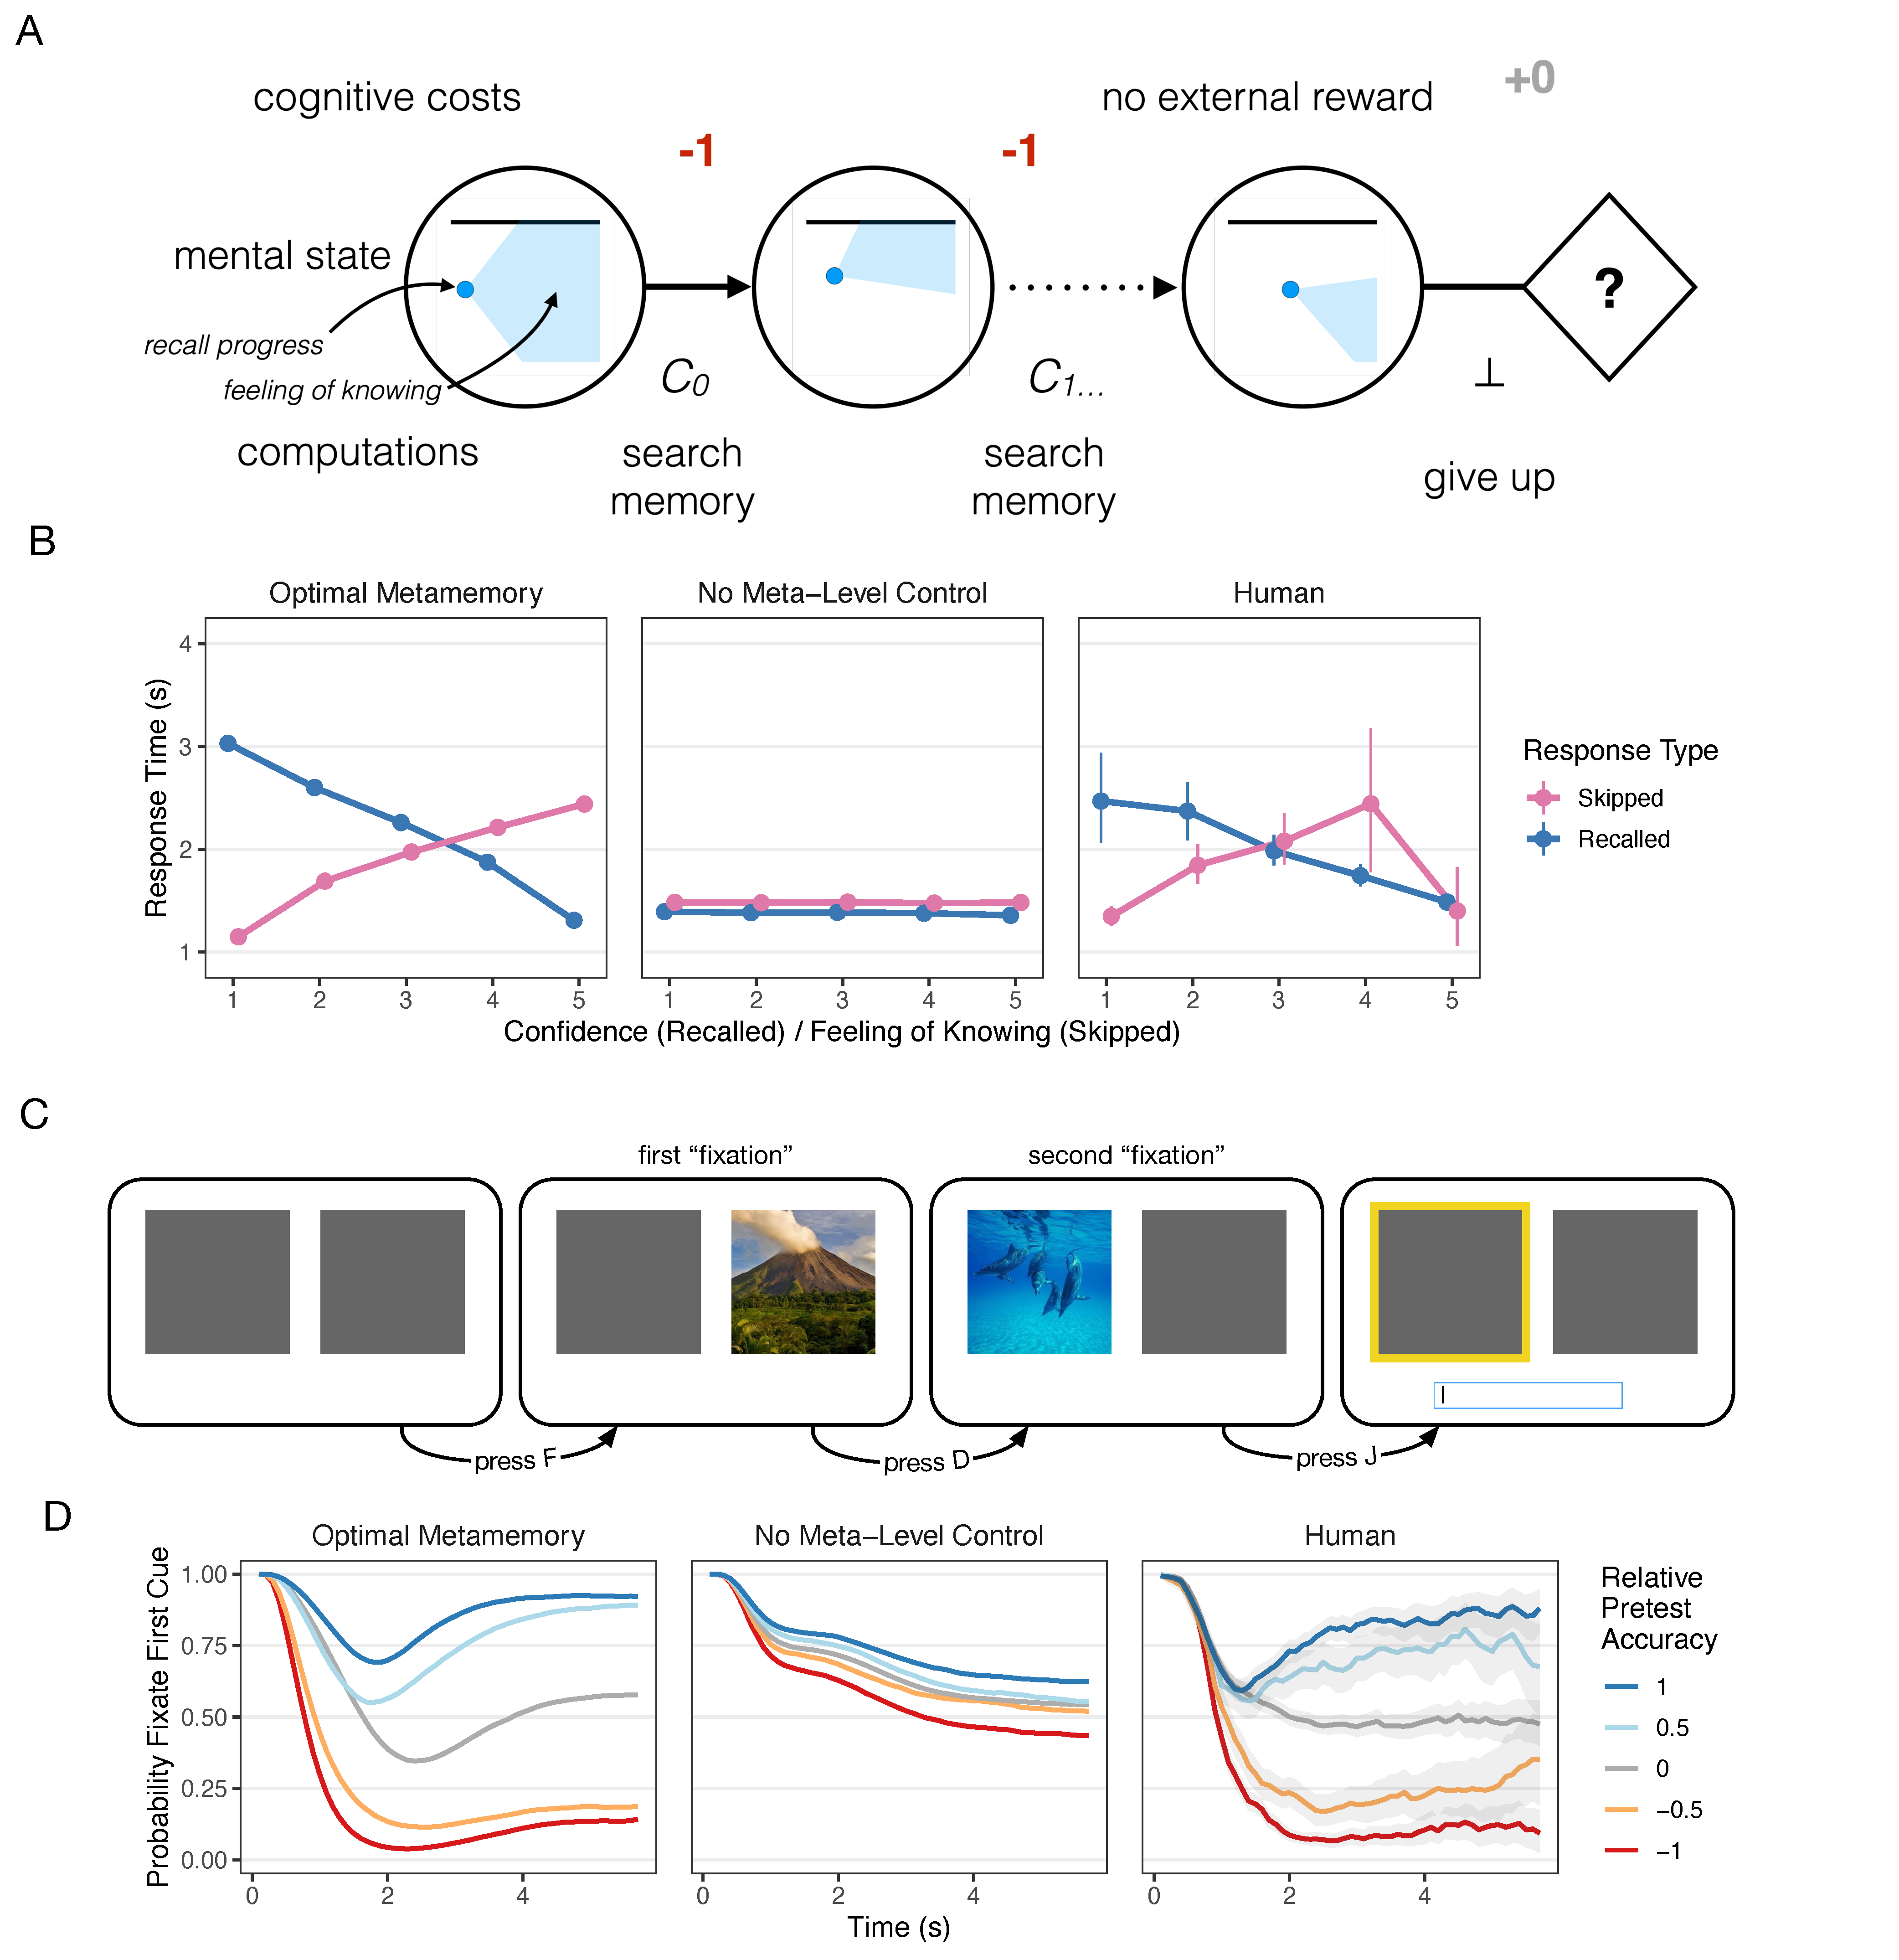
\includegraphics[width=\textwidth]{diagrams/precis/memory.pdf}
  \caption{\captiontitle{Memory}
    \subcap{A} Meta-level MDP. The mental state encodes the current recall progress and an estimate of memory strength (rate of progress). A computation corresponds to searching for the target memory, generating recall progress.
    \subcap{B} Reaction time as a function of metamemory judgment (feeling of knowing for skip trials, confidence for recall trials), separately for trials in which participants correctly recalled the target vs. skipped without responding. The models' metamemory judgments are made based on the inferred memory strength at the end of the trial.
    \subcap{C} Multiple-cued recall task. Participants were presented with two images on each trial and could recall the word associated with either of them. Only one cue was visible at a time; participants could flip between them with the D and F keys. At any point they could press J or K to select an image for recall.
    \subcap{D} Timecourse of attention to the first cue, split by its memory strength (operationalized by accuracy in the pretest phase).
  }
  \label{fig:memory}
\end{figure}


Consider next the all-too-familiar situation of running into someone whose name you cannot recall. If it feels as though the name is about to come to you, you may pause before saying hello. But every moment you delay only exacerbates the awkwardness of the situation. \textbf{How do people know when to stop searching for a memory?}

Most empirical work on metacognition in the domain of memory (or ``metamemory'') has focused on how people are able to monitor their memory states \citep{reder1992determines,eakin2005illusions} and on evaluating the accuracy of those judgments \citep{hart1965memory,vesonder1985ability,dunlosky2007metacomprehension}. Less emphasis, however, has been placed on understanding the function of metamemory judgments \citep{schwartz2017metamemory}. In a highly influential paper, \citet{nelson1990metamemory} proposed that the function of metacognitive systems is to allow effective control of ongoing cognition. For example, they outlined a theory in which a dynamically updated feeling of knowing is used to inform the decision of when to terminate an unsuccessful recall attempt. However, despite this early progress, previous work has not proposed a computational model of how these feeling of knowing estimates might be dynamically generated, nor of how they could be used to control recall efforts. 

In this chapter, I provide such a model, formalizing the decision of when to terminate a memory search as a metalevel MDP (\figref{fig:memory}{a}). Here, the mental states capture the amount of progress one has made towards recalling a memory as well as a metacognitive estimate of the rate of progress (that is, a ``feeling of knowing'' \citealp{hart1965memory}). The computations correspond to continuing to search for the target. The transition function describes how recall progress noisily accumulates through search. Finally, the reward function encodes the value of recalling the item (when a threshold level of progress is reached) and a fixed cost for each moment spent searching.

Solving this metalevel MDP reveals that it is optimal to quickly abandon an attempt to recall a weak memory, one for which recall progresses slowly. The model thus captures the consistent empirical finding that people search longer before giving up on memories that they report having a higher feeling of knowing for \citealp{nelson1984comparison,nhouyvanisvong1998rapid,gruneberg1977methodological,lachman1979metamemory}. In one striking demonstration of this phenomenon, \citet{costermans1992confidence} found opposite relationships between judgments of memory strength and response time when the item was recalled vs. not recalled: people gave high confidence judgments for items that were recalled quickly but low feeling-of-knowing judgments for items that were skipped quickly. As shown in \figref{fig:memory}{b}, the optimal model reproduces this pattern, while a model without meta-level control (but the same underlying memory recall process) fails to capture either effect.

One weakness with the above finding, and indeed with many empirical results in metamemory, is that we observe at most one single metacognitive decision in each trial, the decision to terminate search. To provide a stronger test of the sequential search-evaluate loop, my colleagues and I designed a modified cued-recall paradigm in which two candidate memories could be recalled on each trial (\figref{fig:memory}{c}). By tracking attention to the corresponding cues using a keypress-contingent display, we could observe this metacognitive process unfolding even before a memory was recalled or given up on. Interestingly, \figref{fig:memory}{d} shows that, contrary to the decision-making case studied in the previous chapter, the optimal policy preferentially attends to cues associated with stronger memories even when there are only two options. Participants showed the same pattern. This provides strong evidence that people can estimate the strength of a memory before recalling it, and use that information to guide their recall efforts. To our knowledge, it is also the first quantitative demonstration of a metamemory process unfolding over time.

% This chapter is based on a preprint that is currently under review at \emph{Psychological Review}.

\section{Chapter 5: Planning}

\begin{figure}[ph]
  \centering
  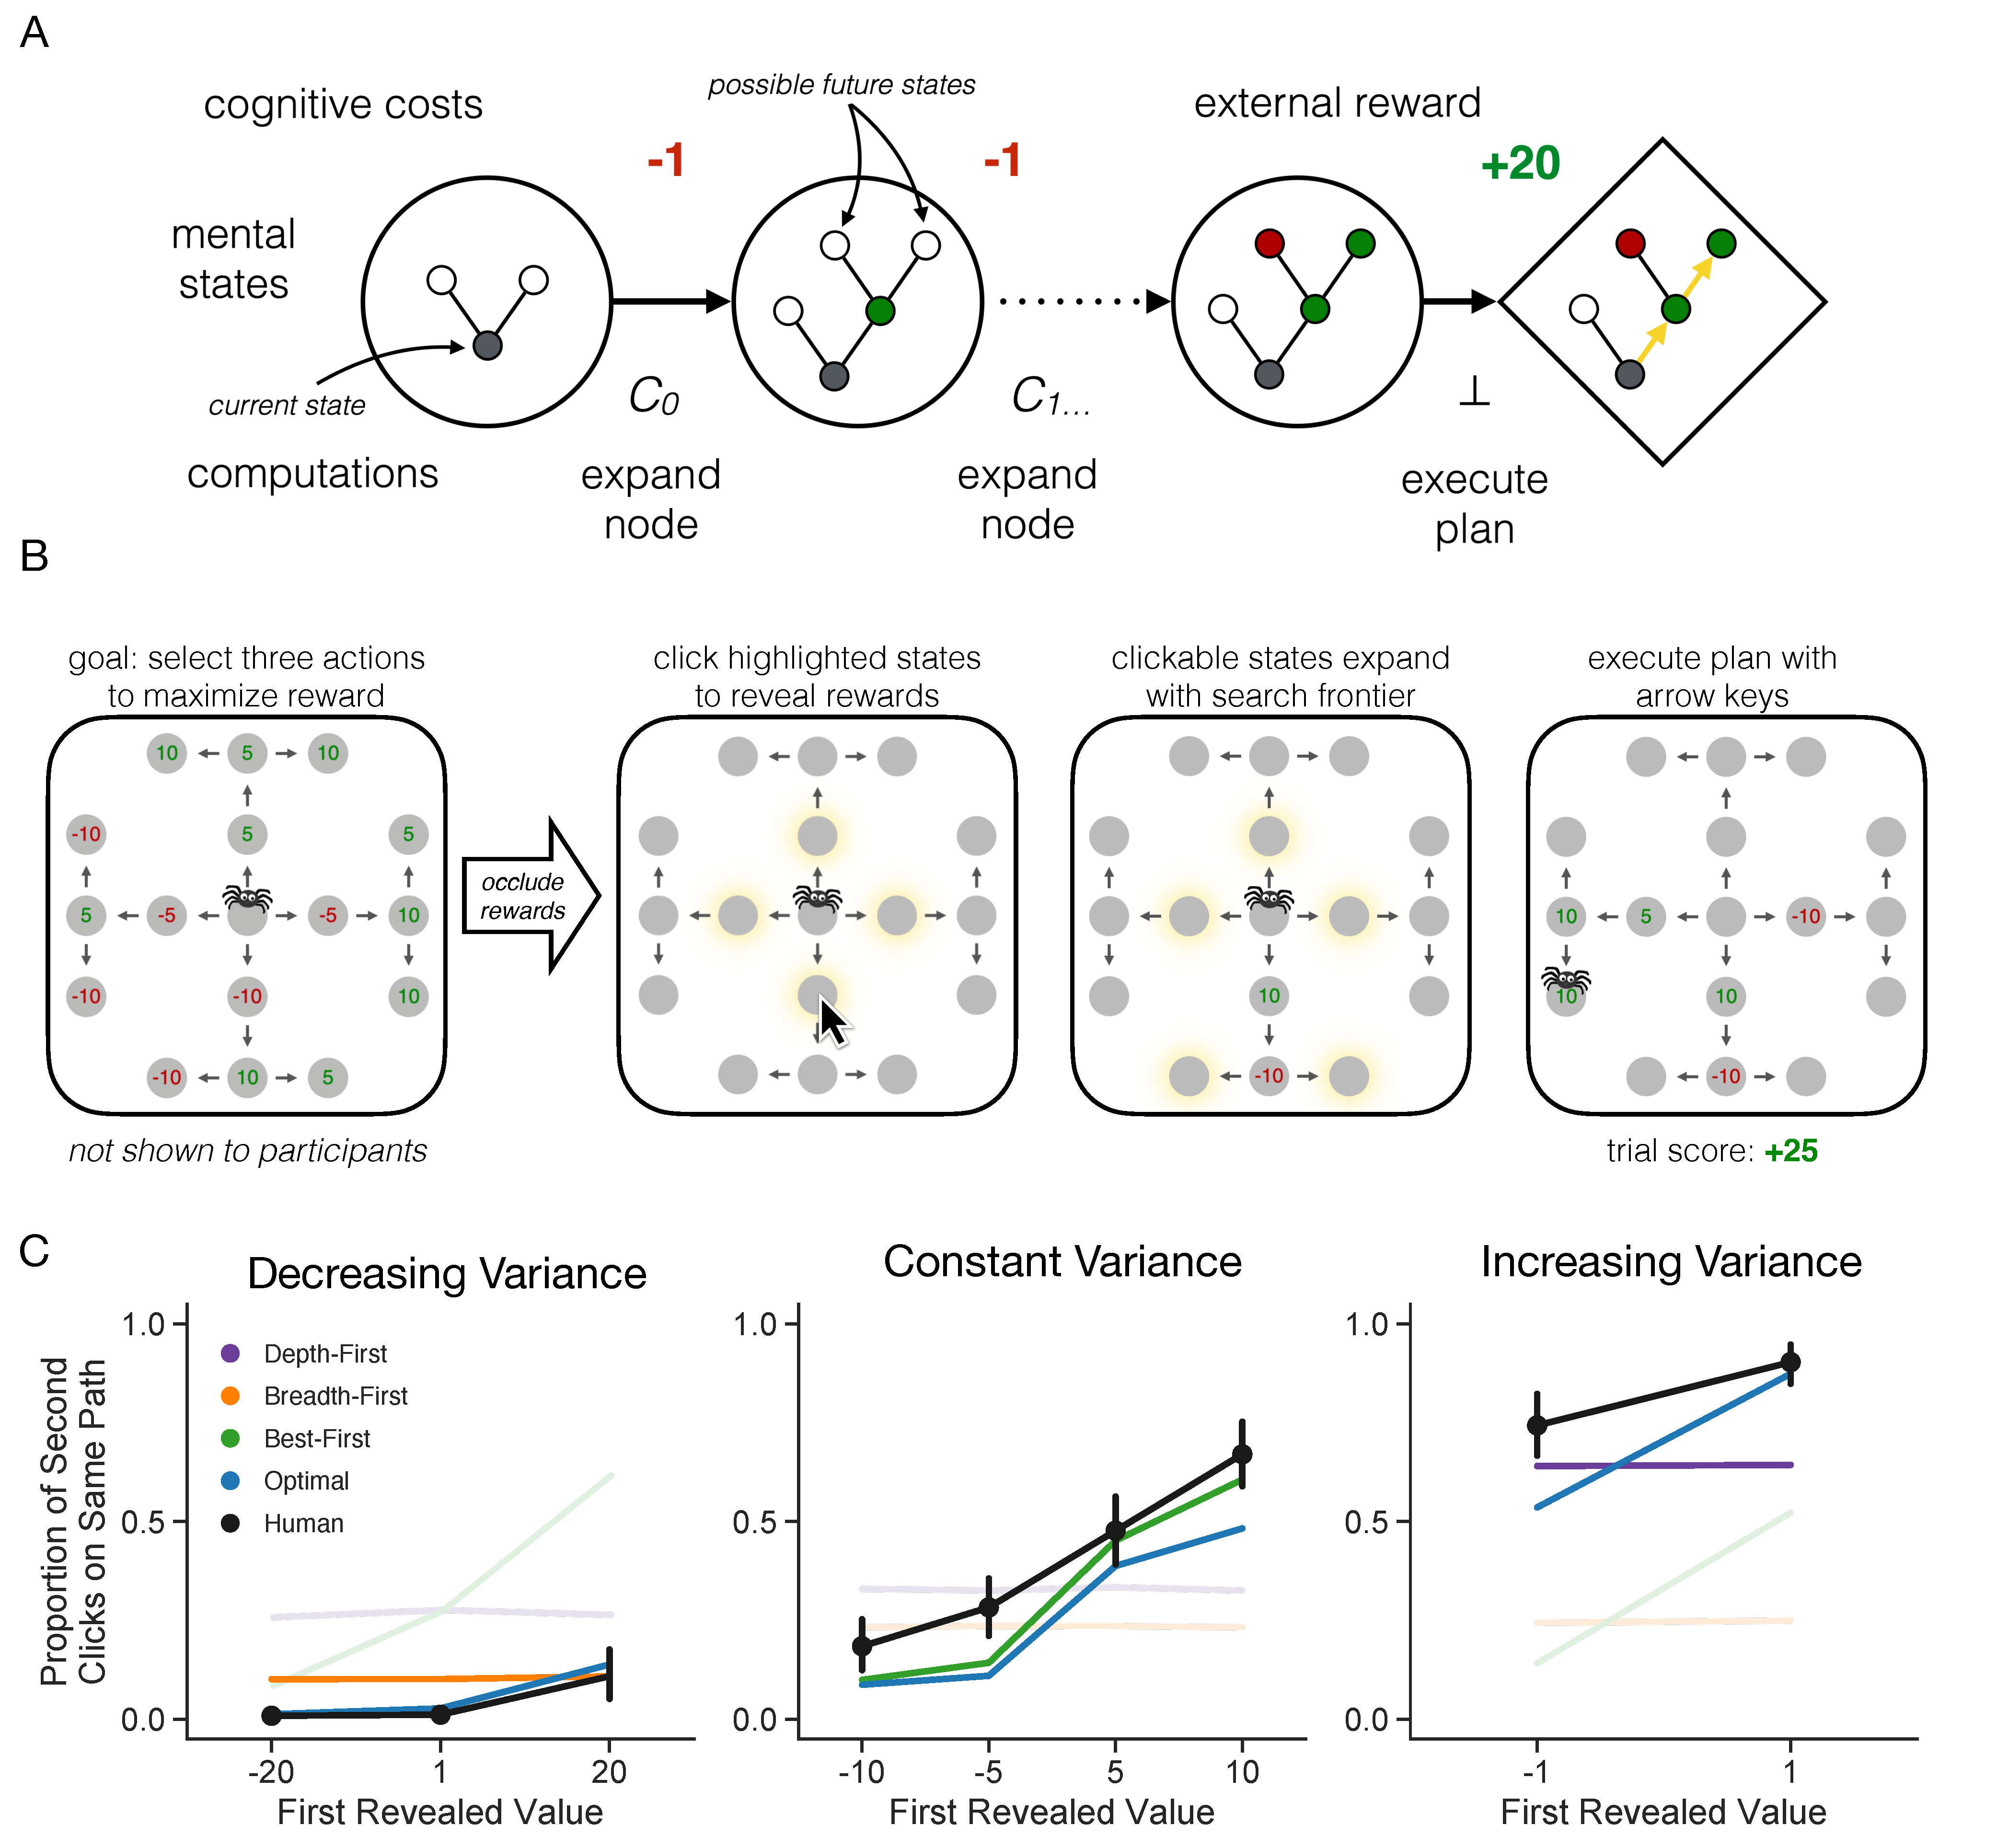
\includegraphics[width=\textwidth]{diagrams/precis/planning.pdf}
  \caption{\captiontitle{Planning}
    \subcap{A} Meta-level MDP. The mental state is a decision-tree, which represents possible future actions (edges), states (nodes), and rewards (green/red). A computation corresponds to considering a future state and expanding the decision tree.
    \subcap{B} Experimental task. The internal process of expanding a decision tree is externalized by forcing participants to click to reveal the reward to be gained at each state.
    \subcap{C} Adaptation of planning strategy in environments with different reward structures (see main text). Each panel shows the probability of making a second click on the same path as the first click, depending on the value revealed by that first click. Models that achieve high reward in the environment are highlighted. % Modulating the distribution of rewards in the environment changes the optimal planning stategy: breadth-first when large rewards are near the initial state, best-first when they are distributed evenly, and depth-first when they are far from the initial state.
  }
  \label{fig:planning}
\end{figure}


Finally, consider the problem faced by a traveler in an unfamiliar country, deciding which cities to visit. Geographical concerns limit which cities they can travel between, so their first stop will shape the whole trip. But there are far too many possible routes to consider every one. \textbf{How do we know which hypothetical courses of action to evaluate, and which to ignore?}

How people solve problems that require thinking multiple steps ahead has been a focal question since the very earliest attempts to understand the human mind in computational terms \citep{newell1956logic,newell1972human}. Both then and now, most work on human planning has focused on identifying the heuristics people use to circumvent the intractability of exhaustive planning. For example, people might limit the depth of their search \citep{macgregor2001information,keramati2016adaptive,krusche2018adaptive,snider2015prospective}, ``prune'' away initially unpromising courses of action \citep{huys2012bonsai,huys2015interplay}, or avoid planning altogether by relying on habit or ``memoization'' \citep{huys2015interplay,kool2017costbenefit}. However, the questions of why people use those particular heuristics and of predicting which of the many possible heuristics people will employ in any particular case, have been relatively unexplored.

To provide a normative theory of planning under computational constraints, we can model planning---specifically, decision tree search---as a metalevel MDP (\figref{fig:planning}{a}). A mental state corresponds to a partially constructed decision tree, which represents possible sequences of actions and outcomes as a tree-structured graph. A computation corresponds to \emph{node expansion}; this operation determines the cost or reward for visiting a state, integrates that value into the total value of the path leading to that state, and adds the immediate successors of the target state to the search frontier, that is, the set of nodes that can be expanded on the next iteration. The transition function encodes these dynamics---critically, it also encodes prior information the agent may have about where large rewards are likely to be found. Finally, the metalevel reward function assigns a fixed cost for each node expansion operation; and when the agent terminates planning, they receive a reward equal to the expected value of the external rewards that will be gained by executing a plan chosen with the current decision tree.

Solving this metalevel MDP yields an optimal planning algorithm. But how can we compare this algorithm to human planning, given that the latter takes place entirely inside a person's head? To circumvent this challenge, my colleagues and I designed a task that makes people's planning directly observable (\figref{fig:planning}{b}). Inspired by the classic Mouselab paradigm \citep{payne1988adaptive}, our task externalizes planning operations as information-gathering actions. Specifically, participants must click future states to see what reward they would gain if they visited that state. The sequence of clicks thus reveals the order in which the participant considered each state. This allows us to evaluate candidate models at the level of individual node expansion operations, providing a stronger and more objective test than is possible with previous approaches based on model comparison over the actions people take (e.g., \citealp{huys2015interplay,vanopheusden2017computational}) or verbal reports of their planning process (e.g., \citealp{degroot1965thought,newell1972human}).

% In an unstructured environment (Experiment 1), the optimal planning strategy closely resembles best-first search with a stopping rule that is sensitive to both absolute and relative value; that is, it generally expands nodes on the path that has maximal expected value under the current decision tree and it commits to a plan when it finds one whose expected value is high and/or better than competing plans. A heuristic model designed to capture this strategy explains participants' clicks better than any combination of previously proposed heuristic planning mechanisms such as best-first search and pruning. However, the optimal model still predicts behavior best, achieving the highest out-of-sample likelihood.

While I have emphasized adaptation to internal environments, our cognitive processes are also shaped by the external environment. To investigate this kind of adaptation, we constructed three environments with different reward distributions. In the ``constant variance'' environment, all states had the same reward distribution. In the other two environments, most states had small rewards and extreme rewards could only be found in one state on each path: the first state in the ``decreasing variance'' environment and the last state in the ``increasing variance'' environment. We designed these environments such that the optimal planning algorithm resembled a different classical algorithm in each case: breadth-first for decreasing variance, best-first for constant variance, and depth-first for increasing variance. Our participants appeared to adapt their planning strategies accordingly, as revealed by the frequency with which they continued down the first-clicked path with their second click (\figref{fig:planning}{c}), doing so rarely in the decreasing variance case (like breadth-first), frequently in the increasing variance case (like depth-first), and only after revealing a large reward in the constant variance case (like best-first). Although one heuristic model in each condition resembles the behavioral pattern, only the optimal model could capture behavior in all three conditions. 

 % shows a simple behavioral marker of this adaptation. Considering only trials on which at least two clicks were made, we ask how often people use their second click to continue down the path that they began with their first, depending on the value revealed by that first click. An overall tendency to continue down the same path is consistent with a depth-first strategy, the reverse tendency is consistent with a breadth-first strategy, and high sensitivity to the revealed value is consistent with a best-first strategy. We see that both people and the optimal model adjust their strategy in the different environments, as predicted. Although one heuristic model in each condition resembles the pattern shown by humans and the optimal model, no single heuristic model could capture behavior in all conditions. 

So far, I have focused on the cases where people resemble the optimal model. However, we also found systematic deviations from optimal planning. Most notably, when we removed the search-frontier constraint (highlighted states in \figref{fig:planning}{b}) in Experiments 3 and 4, we found a strong bias towards considering states in the order in which they would be traversed. This suggests that our metalevel MDP does not capture all the factors constraining human planning in naturalistic settings. In particular, in many cases people may not be able to sample arbitrary future states, and when they can they may have access to a generative model that makes it easier to simulate in temporal order than to reason backwards from effect to cause. If people's planning algorithms are adapted to the naturalistic case, we would expect to see discrepancies when these important constraints are removed. This highlights another key strength of rational models: the cases where theg model is ``wrong'' can be just as---if not more---informative than the cases where it's right.

This work was published in \emph{Nature Human Behavior} \citep{callaway2022rational}.


\section{Chapter 6: Conclusion}

% Across all three domains, my dissertation research shows how Simon's 1955 insight---that cognitive processes are shaped by the environments both within and outside the mind---can be formalized to generate rational mechanistic models that explain both how and why cognitive processes are the way they are.

In the final chapter, I discuss related theoretical approaches and identify four key directions in which the metalevel MDP framework could be extended in future work: (1) metalevel reinforcement learning, (2) incomplete or imperfect metacognition, (3) interleaved computation and action, and (4) optimization of the metalevel MDP itself. I then reflect on the role of frameworks in cognitive science, focusing on the ways in which they constrain our thinking, and emphasizing that these constraints are both a blessing and a curse.

My dissertation presents a general framework for modeling cognition as a sequential decision problem: metalevel Markov decision processes. It shows how the framework can be applied to derive rational mechanistic models in three different domains: attention, memory, and planning. And in each case, we find that human behavior showed substantial qualitative alignment with the optimal metalevel policy. Taken together, the results suggest that human cognitive processes are well-adapted to the internal environments in which they operate. More importantly, by formally characterizing the problems posed by those mental environments, and their optimal solutions, we develop a richer understanding of human cognition in each of these domains.


\clearpage
\bibliography{references,extra}
\addcontentsline{toc}{chapter}{References}
\bibliographystyle{apalike2}

\end{document}